%%%%%%%%%%%%%%%%%%%%%%%%%%%%%%%%%%%%%%%%%%%%%%%%%%%%%%%%%%%%%%%%%%%%%%%%%%%%%%%%%%%%%%%%%%%%%%%%%
%
% Document:      DM  product tree
%
%%%%%%%%%%%%%%%%%%%%%%%%%%%%%%%%%%%%%%%%%%%%%%%%%%%%%%%%%%%%%%%%%%%%%%%%%%%%%%
\documentclass{article}
\usepackage{times,layouts}
\usepackage{tikz,hyperref,amsmath}
\usetikzlibrary{positioning,arrows,shapes,decorations.shapes,shapes.arrows}
\usetikzlibrary{backgrounds,calc}
\usepackage[paperwidth=25cm,paperheight=150cm,
left=-2mm,top=3mm,bottom=0mm,right=0mm,
noheadfoot,marginparwidth=0pt,includemp=false,
textwidth=30cm,textheight=50mm]{geometry}
\newcommand\showpage{%
\setlayoutscale{0.5}\setlabelfont{\tiny}\printheadingsfalse\printparametersfalse
\currentpage\pagedesign}
\hypersetup{pdftitle={DM organisation }, pdfsubject={Diagram illustrating the
products in LSST DM }, pdfauthor={ William O'Mullane}}
\tikzstyle{wbbox}=[rectangle, rounded corners=3pt, draw=black, top color=blue!50!white, bottom color=white, very thick, minimum height=12mm, inner sep=2pt, text centered, text width=30mm] 
\tikzstyle{pbox}=[rectangle, rounded corners=3pt, draw=black, top color=yellow!50!white, bottom color=white, very thick, minimum height=7mm, inner sep=2pt, text centered, text width=35mm] 
\tikzstyle{pline}=[-, thick]\begin{document}
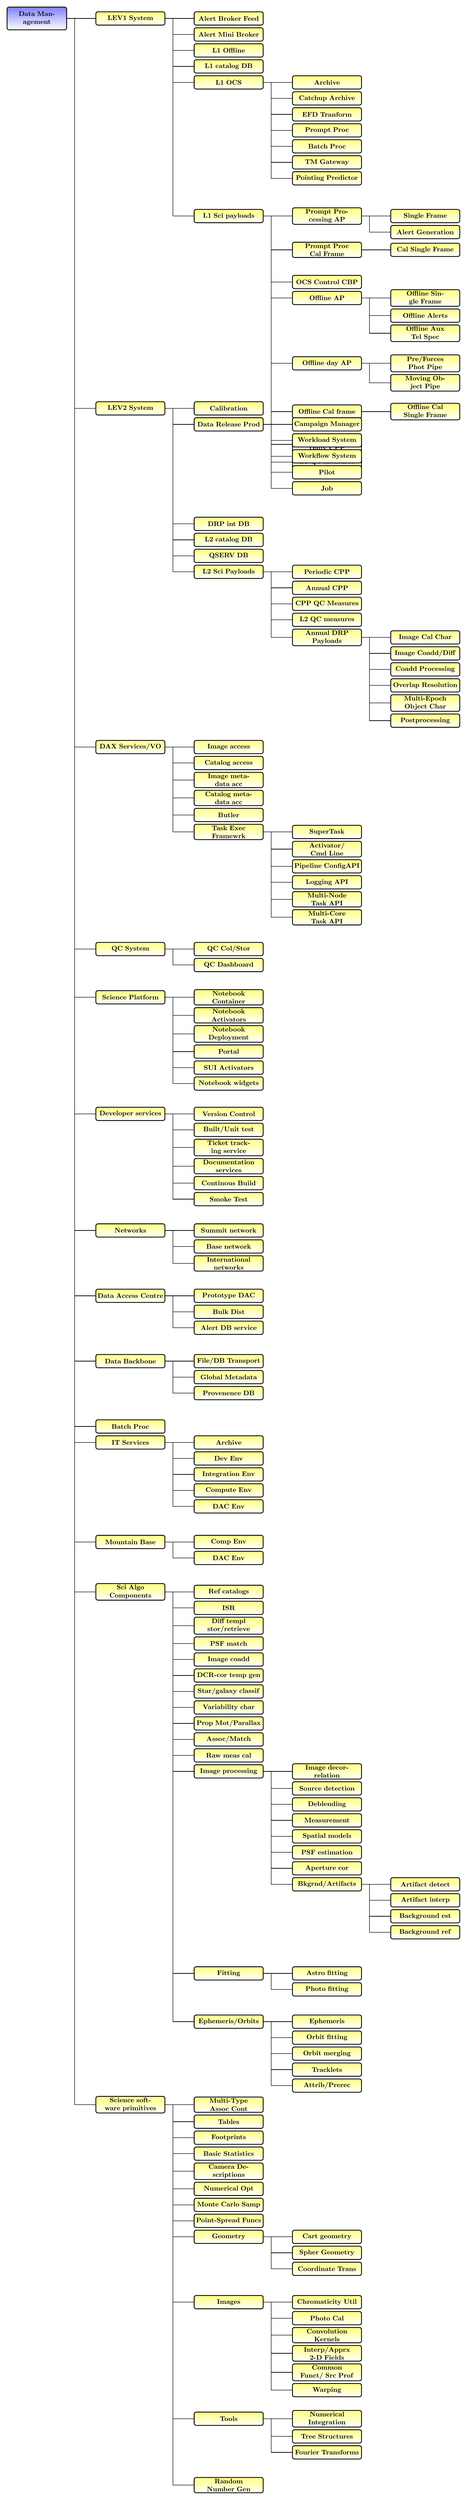
\begin{tikzpicture}[node distance=0mm]
\node (DM) [wbbox]{\textbf{Data Management}}; 
\node (L1) [pbox,right=15mm of DM] {\textbf{LEV1 System}}; 
 \draw[pline] (DM.east) -| ++(0.4,0)  |- (L1.west);
 \node (ABFS) [pbox,right=15mm of L1] {\textbf{Alert Broker Feed}}; 
 \draw[pline] (L1.east) -| ++(0.4,0)  |- (ABFS.west);
 \node (AMBS) [pbox,below=1mm of ABFS] {\textbf{Alert Mini Broker}}; 
 \draw[pline] (L1.east) -| ++(0.4,0)  |- (AMBS.west);
 \node (L1OFF) [pbox,below=1mm of AMBS] {\textbf{L1 Offline}}; 
 \draw[pline] (L1.east) -| ++(0.4,0)  |- (L1OFF.west);
 \node (L1CATDB) [pbox,below=1mm of L1OFF] {\textbf{L1 catalog DB}}; 
 \draw[pline] (L1.east) -| ++(0.4,0)  |- (L1CATDB.west);
 \node (L1OCS) [pbox,below=1mm of L1CATDB] {\textbf{L1 OCS}}; 
 \draw[pline] (L1.east) -| ++(0.4,0)  |- (L1OCS.west);
 \node (ARC) [pbox,right=15mm of L1OCS] {\textbf{Archive}}; 
 \draw[pline] (L1OCS.east) -| ++(0.4,0)  |- (ARC.west);
 \node (CARC) [pbox,below=1mm of ARC] {\textbf{Catchup Archive}}; 
 \draw[pline] (L1OCS.east) -| ++(0.4,0)  |- (CARC.west);
 \node (EFDT) [pbox,below=1mm of CARC] {\textbf{EFD Tranform}}; 
 \draw[pline] (L1OCS.east) -| ++(0.4,0)  |- (EFDT.west);
 \node (PRMP) [pbox,below=1mm of EFDT] {\textbf{Prompt Proc}}; 
 \draw[pline] (L1OCS.east) -| ++(0.4,0)  |- (PRMP.west);
 \node (BP) [pbox,below=1mm of PRMP] {\textbf{Batch Proc}}; 
 \draw[pline] (L1OCS.east) -| ++(0.4,0)  |- (BP.west);
 \node (TMG) [pbox,below=1mm of BP] {\textbf{TM Gateway}}; 
 \draw[pline] (L1OCS.east) -| ++(0.4,0)  |- (TMG.west);
 \node (POINTP) [pbox,below=1mm of TMG] {\textbf{Pointing Predictor}}; 
 \draw[pline] (L1OCS.east) -| ++(0.4,0)  |- (POINTP.west);
 \node (L1SP) [pbox,below=63mm of L1OCS] {\textbf{L1 Sci payloads}}; 
 \draw[pline] (L1.east) -| ++(0.4,0)  |- (L1SP.west);
 \node (L1PP) [pbox,right=15mm of L1SP] {\textbf{Prompt Processing AP}}; 
 \draw[pline] (L1SP.east) -| ++(0.4,0)  |- (L1PP.west);
 \node (SFPP) [pbox,right=15mm of L1PP] {\textbf{Single Frame}}; 
 \draw[pline] (L1PP.east) -| ++(0.4,0)  |- (SFPP.west);
 \node (AGP) [pbox,below=1mm of SFPP] {\textbf{Alert Generation }}; 
 \draw[pline] (L1PP.east) -| ++(0.4,0)  |- (AGP.west);
 \node (PPCF) [pbox,below=9mm of L1PP] {\textbf{Prompt Proc Cal Frame}}; 
 \draw[pline] (L1SP.east) -| ++(0.4,0)  |- (PPCF.west);
 \node (CSFP) [pbox,right=15mm of PPCF] {\textbf{Cal Single Frame }}; 
 \draw[pline] (PPCF.east) -| ++(0.4,0)  |- (CSFP.west);
 \node (OCSCCBP) [pbox,below=9mm of PPCF] {\textbf{OCS Control CBP}}; 
 \draw[pline] (L1SP.east) -| ++(0.4,0)  |- (OCSCCBP.west);
 \node (OFFAP) [pbox,below=1mm of OCSCCBP] {\textbf{Offline  AP}}; 
 \draw[pline] (L1SP.east) -| ++(0.4,0)  |- (OFFAP.west);
 \node (OFFSFP) [pbox,right=15mm of OFFAP] {\textbf{Offline Single Frame}}; 
 \draw[pline] (OFFAP.east) -| ++(0.4,0)  |- (OFFSFP.west);
 \node (OA) [pbox,below=1mm of OFFSFP] {\textbf{Offline Alerts}}; 
 \draw[pline] (OFFAP.east) -| ++(0.4,0)  |- (OA.west);
 \node (OATS) [pbox,below=1mm of OA] {\textbf{Offline Aux Tel Spec}}; 
 \draw[pline] (OFFAP.east) -| ++(0.4,0)  |- (OATS.west);
 \node (OFFDAP) [pbox,below=27mm of OFFAP] {\textbf{Offline day AP}}; 
 \draw[pline] (L1SP.east) -| ++(0.4,0)  |- (OFFDAP.west);
 \node (PFPP) [pbox,right=15mm of OFFDAP] {\textbf{Pre/Forces Phot Pipe}}; 
 \draw[pline] (OFFDAP.east) -| ++(0.4,0)  |- (PFPP.west);
 \node (MOP) [pbox,below=1mm of PFPP] {\textbf{Moving Object Pipe}}; 
 \draw[pline] (OFFDAP.east) -| ++(0.4,0)  |- (MOP.west);
 \node (OFFCAL) [pbox,below=18mm of OFFDAP] {\textbf{Offline Cal frame}}; 
 \draw[pline] (L1SP.east) -| ++(0.4,0)  |- (OFFCAL.west);
 \node (OFFCALSFP) [pbox,right=15mm of OFFCAL] {\textbf{Offline Cal Single Frame}}; 
 \draw[pline] (OFFCAL.east) -| ++(0.4,0)  |- (OFFCALSFP.west);
 \node (OCSBDCPP) [pbox,below=9mm of OFFCAL] {\textbf{OCS Batch Daily CPP}}; 
 \draw[pline] (L1SP.east) -| ++(0.4,0)  |- (OCSBDCPP.west);
 \node (L1QCM) [pbox,below=1mm of OCSBDCPP] {\textbf{L1 QC measures}}; 
 \draw[pline] (L1SP.east) -| ++(0.4,0)  |- (L1QCM.west);
 \node (L2) [pbox,below=198mm of L1] {\textbf{LEV2 System}}; 
 \draw[pline] (DM.east) -| ++(0.4,0)  |- (L2.west);
 \node (CAL) [pbox,right=15mm of L2] {\textbf{Calibration}}; 
 \draw[pline] (L2.east) -| ++(0.4,0)  |- (CAL.west);
 \node (DRP) [pbox,below=1mm of CAL] {\textbf{Data Release Prod}}; 
 \draw[pline] (L2.east) -| ++(0.4,0)  |- (DRP.west);
 \node (CM) [pbox,right=15mm of DRP] {\textbf{Campaign Manager}}; 
 \draw[pline] (DRP.east) -| ++(0.4,0)  |- (CM.west);
 \node (WLS) [pbox,below=1mm of CM] {\textbf{Workload System}}; 
 \draw[pline] (DRP.east) -| ++(0.4,0)  |- (WLS.west);
 \node (WFS) [pbox,below=1mm of WLS] {\textbf{Workflow System}}; 
 \draw[pline] (DRP.east) -| ++(0.4,0)  |- (WFS.west);
 \node (PILOT) [pbox,below=1mm of WFS] {\textbf{Pilot}}; 
 \draw[pline] (DRP.east) -| ++(0.4,0)  |- (PILOT.west);
 \node (JOB) [pbox,below=1mm of PILOT] {\textbf{Job}}; 
 \draw[pline] (DRP.east) -| ++(0.4,0)  |- (JOB.west);
 \node (DRPDB) [pbox,below=45mm of DRP] {\textbf{DRP int DB}}; 
 \draw[pline] (L2.east) -| ++(0.4,0)  |- (DRPDB.west);
 \node (L2CATDB) [pbox,below=1mm of DRPDB] {\textbf{L2 catalog DB}}; 
 \draw[pline] (L2.east) -| ++(0.4,0)  |- (L2CATDB.west);
 \node (QSERV) [pbox,below=1mm of L2CATDB] {\textbf{QSERV DB}}; 
 \draw[pline] (L2.east) -| ++(0.4,0)  |- (QSERV.west);
 \node (L2SP) [pbox,below=1mm of QSERV] {\textbf{L2 Sci Payloads}}; 
 \draw[pline] (L2.east) -| ++(0.4,0)  |- (L2SP.west);
 \node (PCPP) [pbox,right=15mm of L2SP] {\textbf{Periodic CPP}}; 
 \draw[pline] (L2SP.east) -| ++(0.4,0)  |- (PCPP.west);
 \node (ACPP) [pbox,below=1mm of PCPP] {\textbf{Annual CPP}}; 
 \draw[pline] (L2SP.east) -| ++(0.4,0)  |- (ACPP.west);
 \node (CPPQC) [pbox,below=1mm of ACPP] {\textbf{CPP QC Measures}}; 
 \draw[pline] (L2SP.east) -| ++(0.4,0)  |- (CPPQC.west);
 \node (L2QCM) [pbox,below=1mm of CPPQC] {\textbf{L2 QC measures}}; 
 \draw[pline] (L2SP.east) -| ++(0.4,0)  |- (L2QCM.west);
 \node (ADRP) [pbox,below=1mm of L2QCM] {\textbf{Annual DRP Payloads}}; 
 \draw[pline] (L2SP.east) -| ++(0.4,0)  |- (ADRP.west);
 \node (ICC) [pbox,right=15mm of ADRP] {\textbf{Image Cal Char}}; 
 \draw[pline] (ADRP.east) -| ++(0.4,0)  |- (ICC.west);
 \node (ICADIF) [pbox,below=1mm of ICC] {\textbf{Image Coadd/Diff}}; 
 \draw[pline] (ADRP.east) -| ++(0.4,0)  |- (ICADIF.west);
 \node (COADDP) [pbox,below=1mm of ICADIF] {\textbf{Coadd Processing}}; 
 \draw[pline] (ADRP.east) -| ++(0.4,0)  |- (COADDP.west);
 \node (OVRES) [pbox,below=1mm of COADDP] {\textbf{Overlap Resolution}}; 
 \draw[pline] (ADRP.east) -| ++(0.4,0)  |- (OVRES.west);
 \node (MEOC) [pbox,below=1mm of OVRES] {\textbf{Multi-Epoch Object Char}}; 
 \draw[pline] (ADRP.east) -| ++(0.4,0)  |- (MEOC.west);
 \node (POSTP) [pbox,below=1mm of MEOC] {\textbf{Postprocessing}}; 
 \draw[pline] (ADRP.east) -| ++(0.4,0)  |- (POSTP.west);
 \node (DAXS) [pbox,below=171mm of L2] {\textbf{DAX Services/VO}}; 
 \draw[pline] (DM.east) -| ++(0.4,0)  |- (DAXS.west);
 \node (IMA) [pbox,right=15mm of DAXS] {\textbf{Image access}}; 
 \draw[pline] (DAXS.east) -| ++(0.4,0)  |- (IMA.west);
 \node (CATA) [pbox,below=1mm of IMA] {\textbf{Catalog access}}; 
 \draw[pline] (DAXS.east) -| ++(0.4,0)  |- (CATA.west);
 \node (IMMETA) [pbox,below=1mm of CATA] {\textbf{Image metadata acc}}; 
 \draw[pline] (DAXS.east) -| ++(0.4,0)  |- (IMMETA.west);
 \node (CATMETA) [pbox,below=1mm of IMMETA] {\textbf{Catalog metadata acc}}; 
 \draw[pline] (DAXS.east) -| ++(0.4,0)  |- (CATMETA.west);
 \node (BUTL) [pbox,below=1mm of CATMETA] {\textbf{Butler}}; 
 \draw[pline] (DAXS.east) -| ++(0.4,0)  |- (BUTL.west);
 \node (TEF) [pbox,below=1mm of BUTL] {\textbf{Task Exec Framewrk}}; 
 \draw[pline] (DAXS.east) -| ++(0.4,0)  |- (TEF.west);
 \node (SUPT) [pbox,right=15mm of TEF] {\textbf{SuperTask}}; 
 \draw[pline] (TEF.east) -| ++(0.4,0)  |- (SUPT.west);
 \node (ACTI) [pbox,below=1mm of SUPT] {\textbf{Activator/ Cmd Line }}; 
 \draw[pline] (TEF.east) -| ++(0.4,0)  |- (ACTI.west);
 \node (PIPECON) [pbox,below=1mm of ACTI] {\textbf{Pipeline ConfigAPI}}; 
 \draw[pline] (TEF.east) -| ++(0.4,0)  |- (PIPECON.west);
 \node (LOG) [pbox,below=1mm of PIPECON] {\textbf{Logging API}}; 
 \draw[pline] (TEF.east) -| ++(0.4,0)  |- (LOG.west);
 \node (MNTA) [pbox,below=1mm of LOG] {\textbf{Multi-Node Task API}}; 
 \draw[pline] (TEF.east) -| ++(0.4,0)  |- (MNTA.west);
 \node (MCTA) [pbox,below=1mm of MNTA] {\textbf{Multi-Core Task API}}; 
 \draw[pline] (TEF.east) -| ++(0.4,0)  |- (MCTA.west);
 \node (QCS) [pbox,below=99mm of DAXS] {\textbf{QC System}}; 
 \draw[pline] (DM.east) -| ++(0.4,0)  |- (QCS.west);
 \node (QCCS) [pbox,right=15mm of QCS] {\textbf{QC Col/Stor}}; 
 \draw[pline] (QCS.east) -| ++(0.4,0)  |- (QCCS.west);
 \node (QCDASH) [pbox,below=1mm of QCCS] {\textbf{QC Dashboard}}; 
 \draw[pline] (QCS.east) -| ++(0.4,0)  |- (QCDASH.west);
 \node (SCIP) [pbox,below=18mm of QCS] {\textbf{Science Platform}}; 
 \draw[pline] (DM.east) -| ++(0.4,0)  |- (SCIP.west);
 \node (NBC) [pbox,right=15mm of SCIP] {\textbf{Notebook Container}}; 
 \draw[pline] (SCIP.east) -| ++(0.4,0)  |- (NBC.west);
 \node (NBCA) [pbox,below=1mm of NBC] {\textbf{Notebook Activators}}; 
 \draw[pline] (SCIP.east) -| ++(0.4,0)  |- (NBCA.west);
 \node (NDB) [pbox,below=1mm of NBCA] {\textbf{Notebook Deployment}}; 
 \draw[pline] (SCIP.east) -| ++(0.4,0)  |- (NDB.west);
 \node (PORT) [pbox,below=1mm of NDB] {\textbf{Portal}}; 
 \draw[pline] (SCIP.east) -| ++(0.4,0)  |- (PORT.west);
 \node (SUIA) [pbox,below=1mm of PORT] {\textbf{SUI Activators}}; 
 \draw[pline] (SCIP.east) -| ++(0.4,0)  |- (SUIA.west);
 \node (NBW) [pbox,below=1mm of SUIA] {\textbf{Notebook widgets}}; 
 \draw[pline] (SCIP.east) -| ++(0.4,0)  |- (NBW.west);
 \node (DEVS) [pbox,below=54mm of SCIP] {\textbf{Developer services}}; 
 \draw[pline] (DM.east) -| ++(0.4,0)  |- (DEVS.west);
 \node (SVCS) [pbox,right=15mm of DEVS] {\textbf{Version Control}}; 
 \draw[pline] (DEVS.east) -| ++(0.4,0)  |- (SVCS.west);
 \node (SBT) [pbox,below=1mm of SVCS] {\textbf{Built/Unit test }}; 
 \draw[pline] (DEVS.east) -| ++(0.4,0)  |- (SBT.west);
 \node (TICKS) [pbox,below=1mm of SBT] {\textbf{Ticket tracking service}}; 
 \draw[pline] (DEVS.east) -| ++(0.4,0)  |- (TICKS.west);
 \node (DOCS) [pbox,below=1mm of TICKS] {\textbf{Documentation services}}; 
 \draw[pline] (DEVS.east) -| ++(0.4,0)  |- (DOCS.west);
 \node (AINT) [pbox,below=1mm of DOCS] {\textbf{Continous Build}}; 
 \draw[pline] (DEVS.east) -| ++(0.4,0)  |- (AINT.west);
 \node (DEPL) [pbox,below=1mm of AINT] {\textbf{Smoke Test}}; 
 \draw[pline] (DEVS.east) -| ++(0.4,0)  |- (DEPL.west);
 \node (NET) [pbox,below=54mm of DEVS] {\textbf{Networks }}; 
 \draw[pline] (DM.east) -| ++(0.4,0)  |- (NET.west);
 \node (SUMNET) [pbox,right=15mm of NET] {\textbf{Summit network}}; 
 \draw[pline] (NET.east) -| ++(0.4,0)  |- (SUMNET.west);
 \node (BASENET) [pbox,below=1mm of SUMNET] {\textbf{Base network}}; 
 \draw[pline] (NET.east) -| ++(0.4,0)  |- (BASENET.west);
 \node (INTNET) [pbox,below=1mm of BASENET] {\textbf{International networks}}; 
 \draw[pline] (NET.east) -| ++(0.4,0)  |- (INTNET.west);
 \node (DAC) [pbox,below=27mm of NET] {\textbf{Data Access Centre}}; 
 \draw[pline] (DM.east) -| ++(0.4,0)  |- (DAC.west);
 \node (PDAC) [pbox,right=15mm of DAC] {\textbf{Prototype DAC}}; 
 \draw[pline] (DAC.east) -| ++(0.4,0)  |- (PDAC.west);
 \node (BULKD) [pbox,below=1mm of PDAC] {\textbf{Bulk Dist}}; 
 \draw[pline] (DAC.east) -| ++(0.4,0)  |- (BULKD.west);
 \node (ADBS) [pbox,below=1mm of BULKD] {\textbf{Alert DB service}}; 
 \draw[pline] (DAC.east) -| ++(0.4,0)  |- (ADBS.west);
 \node (DBB) [pbox,below=27mm of DAC] {\textbf{Data Backbone}}; 
 \draw[pline] (DM.east) -| ++(0.4,0)  |- (DBB.west);
 \node (DTR) [pbox,right=15mm of DBB] {\textbf{File/DB Transport}}; 
 \draw[pline] (DBB.east) -| ++(0.4,0)  |- (DTR.west);
 \node (GMDS) [pbox,below=1mm of DTR] {\textbf{Global Metadata}}; 
 \draw[pline] (DBB.east) -| ++(0.4,0)  |- (GMDS.west);
 \node (PRDB) [pbox,below=1mm of GMDS] {\textbf{Provenence DB}}; 
 \draw[pline] (DBB.east) -| ++(0.4,0)  |- (PRDB.west);
 \node (BPS) [pbox,below=27mm of DBB] {\textbf{Batch Proc}}; 
 \draw[pline] (DM.east) -| ++(0.4,0)  |- (BPS.west);
 \node (ITS) [pbox,below=1mm of BPS] {\textbf{IT Services}}; 
 \draw[pline] (DM.east) -| ++(0.4,0)  |- (ITS.west);
 \node (ITARC) [pbox,right=15mm of ITS] {\textbf{Archive}}; 
 \draw[pline] (ITS.east) -| ++(0.4,0)  |- (ITARC.west);
 \node (DENV) [pbox,below=1mm of ITARC] {\textbf{Dev Env}}; 
 \draw[pline] (ITS.east) -| ++(0.4,0)  |- (DENV.west);
 \node (INTENV) [pbox,below=1mm of DENV] {\textbf{Integration Env}}; 
 \draw[pline] (ITS.east) -| ++(0.4,0)  |- (INTENV.west);
 \node (COMPENV) [pbox,below=1mm of INTENV] {\textbf{Compute Env}}; 
 \draw[pline] (ITS.east) -| ++(0.4,0)  |- (COMPENV.west);
 \node (DACENV) [pbox,below=1mm of COMPENV] {\textbf{DAC Env}}; 
 \draw[pline] (ITS.east) -| ++(0.4,0)  |- (DACENV.west);
 \node (BASE) [pbox,below=45mm of ITS] {\textbf{Mountain Base}}; 
 \draw[pline] (DM.east) -| ++(0.4,0)  |- (BASE.west);
 \node (BCOMPENV) [pbox,right=15mm of BASE] {\textbf{Comp Env}}; 
 \draw[pline] (BASE.east) -| ++(0.4,0)  |- (BCOMPENV.west);
 \node (BDACENV) [pbox,below=1mm of BCOMPENV] {\textbf{DAC Env}}; 
 \draw[pline] (BASE.east) -| ++(0.4,0)  |- (BDACENV.west);
   no parent 
\node (CSAC) [pbox,below=18mm of BASE] {\textbf{Sci Algo Components}}; 
 \draw[pline] (DM.east) -| ++(0.4,0)  |- (CSAC.west);
 \node (RC) [pbox,right=15mm of CSAC] {\textbf{Ref catalogs}}; 
 \draw[pline] (CSAC.east) -| ++(0.4,0)  |- (RC.west);
 \node (ISR) [pbox,below=1mm of RC] {\textbf{ISR}}; 
 \draw[pline] (CSAC.east) -| ++(0.4,0)  |- (ISR.west);
 \node (DTSR) [pbox,below=1mm of ISR] {\textbf{Diff templ stor/retrieve}}; 
 \draw[pline] (CSAC.east) -| ++(0.4,0)  |- (DTSR.west);
 \node (PSFM) [pbox,below=1mm of DTSR] {\textbf{PSF match}}; 
 \draw[pline] (CSAC.east) -| ++(0.4,0)  |- (PSFM.west);
 \node (IMCOADD) [pbox,below=1mm of PSFM] {\textbf{Image coadd}}; 
 \draw[pline] (CSAC.east) -| ++(0.4,0)  |- (IMCOADD.west);
 \node (DCRCORTMPL) [pbox,below=1mm of IMCOADD] {\textbf{DCR-cor temp gen}}; 
 \draw[pline] (CSAC.east) -| ++(0.4,0)  |- (DCRCORTMPL.west);
 \node (CLASIF) [pbox,below=1mm of DCRCORTMPL] {\textbf{Star/galaxy classif}}; 
 \draw[pline] (CSAC.east) -| ++(0.4,0)  |- (CLASIF.west);
 \node (VARI) [pbox,below=1mm of CLASIF] {\textbf{Variability char}}; 
 \draw[pline] (CSAC.east) -| ++(0.4,0)  |- (VARI.west);
 \node (PMPAR) [pbox,below=1mm of VARI] {\textbf{Prop Mot/Parallax}}; 
 \draw[pline] (CSAC.east) -| ++(0.4,0)  |- (PMPAR.west);
 \node (ASOCMAT) [pbox,below=1mm of PMPAR] {\textbf{Assoc/Match}}; 
 \draw[pline] (CSAC.east) -| ++(0.4,0)  |- (ASOCMAT.west);
 \node (RAWM) [pbox,below=1mm of ASOCMAT] {\textbf{Raw meas cal}}; 
 \draw[pline] (CSAC.east) -| ++(0.4,0)  |- (RAWM.west);
 \node (IMPROC) [pbox,below=1mm of RAWM] {\textbf{Image processing}}; 
 \draw[pline] (CSAC.east) -| ++(0.4,0)  |- (IMPROC.west);
 \node (IMDECOR) [pbox,right=15mm of IMPROC] {\textbf{Image decorrelation}}; 
 \draw[pline] (IMPROC.east) -| ++(0.4,0)  |- (IMDECOR.west);
 \node (SRCD) [pbox,below=1mm of IMDECOR] {\textbf{Source detection}}; 
 \draw[pline] (IMPROC.east) -| ++(0.4,0)  |- (SRCD.west);
 \node (DEBL) [pbox,below=1mm of SRCD] {\textbf{Deblending}}; 
 \draw[pline] (IMPROC.east) -| ++(0.4,0)  |- (DEBL.west);
 \node (MEAS) [pbox,below=1mm of DEBL] {\textbf{Measurement}}; 
 \draw[pline] (IMPROC.east) -| ++(0.4,0)  |- (MEAS.west);
 \node (SPATM) [pbox,below=1mm of MEAS] {\textbf{Spatial models}}; 
 \draw[pline] (IMPROC.east) -| ++(0.4,0)  |- (SPATM.west);
 \node (PSFE) [pbox,below=1mm of SPATM] {\textbf{PSF estimation}}; 
 \draw[pline] (IMPROC.east) -| ++(0.4,0)  |- (PSFE.west);
 \node (APCOR) [pbox,below=1mm of PSFE] {\textbf{Aperture cor}}; 
 \draw[pline] (IMPROC.east) -| ++(0.4,0)  |- (APCOR.west);
 \node (BGART) [pbox,below=1mm of APCOR] {\textbf{Bkgrnd/Artifacts}}; 
 \draw[pline] (IMPROC.east) -| ++(0.4,0)  |- (BGART.west);
 \node (ADET) [pbox,right=15mm of BGART] {\textbf{Artifact detect}}; 
 \draw[pline] (BGART.east) -| ++(0.4,0)  |- (ADET.west);
 \node (AINT) [pbox,below=1mm of ADET] {\textbf{Artifact interp}}; 
 \draw[pline] (BGART.east) -| ++(0.4,0)  |- (AINT.west);
 \node (BGE) [pbox,below=1mm of AINT] {\textbf{Background est}}; 
 \draw[pline] (BGART.east) -| ++(0.4,0)  |- (BGE.west);
 \node (BGR) [pbox,below=1mm of BGE] {\textbf{Background ref}}; 
 \draw[pline] (BGART.east) -| ++(0.4,0)  |- (BGR.west);
 \node (FIT) [pbox,below=99mm of IMPROC] {\textbf{Fitting}}; 
 \draw[pline] (CSAC.east) -| ++(0.4,0)  |- (FIT.west);
 \node (ASTROF) [pbox,right=15mm of FIT] {\textbf{Astro fitting}}; 
 \draw[pline] (FIT.east) -| ++(0.4,0)  |- (ASTROF.west);
 \node (PHOTF) [pbox,below=1mm of ASTROF] {\textbf{Photo fitting}}; 
 \draw[pline] (FIT.east) -| ++(0.4,0)  |- (PHOTF.west);
 \node (ORB) [pbox,below=18mm of FIT] {\textbf{Ephemeris/Orbits}}; 
 \draw[pline] (CSAC.east) -| ++(0.4,0)  |- (ORB.west);
 \node (EPHEM) [pbox,right=15mm of ORB] {\textbf{Ephemeris }}; 
 \draw[pline] (ORB.east) -| ++(0.4,0)  |- (EPHEM.west);
 \node (ORBF) [pbox,below=1mm of EPHEM] {\textbf{Orbit fitting}}; 
 \draw[pline] (ORB.east) -| ++(0.4,0)  |- (ORBF.west);
 \node (ORBM) [pbox,below=1mm of ORBF] {\textbf{Orbit merging}}; 
 \draw[pline] (ORB.east) -| ++(0.4,0)  |- (ORBM.west);
 \node (TRACKL) [pbox,below=1mm of ORBM] {\textbf{Tracklets}}; 
 \draw[pline] (ORB.east) -| ++(0.4,0)  |- (TRACKL.west);
 \node (ATTPREC) [pbox,below=1mm of TRACKL] {\textbf{Attrib/Prerec}}; 
 \draw[pline] (ORB.east) -| ++(0.4,0)  |- (ATTPREC.west);
 \node (SSP) [pbox,below=261mm of CSAC] {\textbf{Science software primitives}}; 
 \draw[pline] (DM.east) -| ++(0.4,0)  |- (SSP.west);
 \node (MTAC) [pbox,right=15mm of SSP] {\textbf{Multi-Type Assoc Cont}}; 
 \draw[pline] (SSP.east) -| ++(0.4,0)  |- (MTAC.west);
 \node (TAB) [pbox,below=1mm of MTAC] {\textbf{Tables}}; 
 \draw[pline] (SSP.east) -| ++(0.4,0)  |- (TAB.west);
 \node (FOOTP) [pbox,below=1mm of TAB] {\textbf{Footprints}}; 
 \draw[pline] (SSP.east) -| ++(0.4,0)  |- (FOOTP.west);
 \node (BSTAT) [pbox,below=1mm of FOOTP] {\textbf{Basic Statistics}}; 
 \draw[pline] (SSP.east) -| ++(0.4,0)  |- (BSTAT.west);
 \node (CAMDES) [pbox,below=1mm of BSTAT] {\textbf{Camera Descriptions}}; 
 \draw[pline] (SSP.east) -| ++(0.4,0)  |- (CAMDES.west);
 \node (NUMOPT) [pbox,below=1mm of CAMDES] {\textbf{Numerical Opt}}; 
 \draw[pline] (SSP.east) -| ++(0.4,0)  |- (NUMOPT.west);
 \node (MCSAMP) [pbox,below=1mm of NUMOPT] {\textbf{Monte Carlo Samp}}; 
 \draw[pline] (SSP.east) -| ++(0.4,0)  |- (MCSAMP.west);
 \node (PSF) [pbox,below=1mm of MCSAMP] {\textbf{Point-Spread Funcs}}; 
 \draw[pline] (SSP.east) -| ++(0.4,0)  |- (PSF.west);
 \node (GEOM) [pbox,below=1mm of PSF] {\textbf{Geometry}}; 
 \draw[pline] (SSP.east) -| ++(0.4,0)  |- (GEOM.west);
 \node (CARTG) [pbox,right=15mm of GEOM] {\textbf{Cart geometry}}; 
 \draw[pline] (GEOM.east) -| ++(0.4,0)  |- (CARTG.west);
 \node (SPHERG) [pbox,below=1mm of CARTG] {\textbf{Spher Geometry}}; 
 \draw[pline] (GEOM.east) -| ++(0.4,0)  |- (SPHERG.west);
 \node (COORDT) [pbox,below=1mm of SPHERG] {\textbf{Coordinate Trans}}; 
 \draw[pline] (GEOM.east) -| ++(0.4,0)  |- (COORDT.west);
 \node (IMAGES) [pbox,below=27mm of GEOM] {\textbf{Images}}; 
 \draw[pline] (SSP.east) -| ++(0.4,0)  |- (IMAGES.west);
 \node (CHROM) [pbox,right=15mm of IMAGES] {\textbf{Chromaticity Util}}; 
 \draw[pline] (IMAGES.east) -| ++(0.4,0)  |- (CHROM.west);
 \node (PHOTOCAL) [pbox,below=1mm of CHROM] {\textbf{Photo Cal}}; 
 \draw[pline] (IMAGES.east) -| ++(0.4,0)  |- (PHOTOCAL.west);
 \node (CONVK) [pbox,below=1mm of PHOTOCAL] {\textbf{Convolution Kernels}}; 
 \draw[pline] (IMAGES.east) -| ++(0.4,0)  |- (CONVK.west);
 \node (IA2DF) [pbox,below=1mm of CONVK] {\textbf{Interp/Apprx 2-D Fields}}; 
 \draw[pline] (IMAGES.east) -| ++(0.4,0)  |- (IA2DF.west);
 \node (CFSRCP) [pbox,below=1mm of IA2DF] {\textbf{Common Funct/ Src Prof}}; 
 \draw[pline] (IMAGES.east) -| ++(0.4,0)  |- (CFSRCP.west);
 \node (WARP) [pbox,below=1mm of CFSRCP] {\textbf{Warping}}; 
 \draw[pline] (IMAGES.east) -| ++(0.4,0)  |- (WARP.west);
 \node (TOOLS) [pbox,below=54mm of IMAGES] {\textbf{Tools}}; 
 \draw[pline] (SSP.east) -| ++(0.4,0)  |- (TOOLS.west);
 \node (NUMI) [pbox,right=15mm of TOOLS] {\textbf{Numerical Integration}}; 
 \draw[pline] (TOOLS.east) -| ++(0.4,0)  |- (NUMI.west);
 \node (TREE) [pbox,below=1mm of NUMI] {\textbf{Tree Structures}}; 
 \draw[pline] (TOOLS.east) -| ++(0.4,0)  |- (TREE.west);
 \node (FT) [pbox,below=1mm of TREE] {\textbf{Fourier Transforms}}; 
 \draw[pline] (TOOLS.east) -| ++(0.4,0)  |- (FT.west);
 \node (RND) [pbox,below=27mm of TOOLS] {\textbf{Random Number Gen}}; 
 \draw[pline] (SSP.east) -| ++(0.4,0)  |- (RND.west);
 \end{tikzpicture}
\end{document}
